\section{Experimental results}
\label{sec:bench}
In this section, we present \rerl an implementation of our proposed approach and its evaluation in terms of (1) accuracy of avoiding bad states and, (2) compile and runtime efficiency. 
\subsection{Implementation}
\rerl is an implementation of our method with several modules. The implementation is available at \href{http://staff.aub.edu.lb/~mj54/rerl}{http://staff.aub.edu.lb/\~{}mj54/rerl}. 
\rerl~ is equipped with a command line interface that accepts a set of configuration options. 
It takes the name of the input BIP file, a file containing the bad states (explicitly or symbolically) to be avoided,  and optional flags (e.g., discount factor, number of episodes, horizon length), and it automatically generates a C++ implementation of the input BIP system embedded with a policy to avoid bad states. 
\begin{lstlisting}[language=Bash]
> java -jar RERL.jar [options] input.bip output.cpp badStates.txt
\end{lstlisting}

\subsection{Evaluation}
\paragraph{Dining philosophers.} Figure~\ref{fig:diningbench} shows an example of dining philosophers modeled in BIP that may deadlock. A deadlock will arise when philosopher $P_0$ allocates its right fork $F_0$, then philosopher $P_1$ allocates its right fork $F_1$. That is, a deadlock state is defined as the concatenation when all the philosophers allocate their right forks. We used \rerl to enforce deadlock freedom on this example. We vary the number of philosophers from $2$ to $47$ increasing by $5$. The total number of states is equal to $6^{n}$, where $n$ is the number of philosophers. 
Clearly, value iteration method would explode when the number of philosophers is greater than $12$. 
%
As for the deep value iteration, we ran it with $50$ \texttt{epochs}, $50$ hidden neuron units and $5$ as degree of fairness. The degree of fairness was chosen to be consistent with the good ($+1$) and bad reward ($-1$). Then, we run the system until it executes $10^5$ iterations. The normal implementation always enters the deadlock state whereas when we apply deep value iteration the obtained implementation always avoid the deadlock state.  
%
\begin{figure}[t]
\centering
\subfigure[Philosopher\label{fig:philo}]{\scalebox{0.55}{\input{figs/philo.pdf_t}}}
\subfigure[Fork\label{fig:fork}]{\scalebox{0.55}{\input{figs/fork.pdf_t}}}
\subfigure[Dining philosophers in BIP\label{fig:dining}]{\scalebox{0.7}{\input{figs/diningbip-deadlock.pdf_t}}} 
\caption{Dining philosophers with possible deadlock.}
\label{fig:diningbench}
\end{figure}
%
We also evaluated the runtime overhead induced by the policy, which at every computation step needs to do a forward propagation on the trained neural network to select the best next interactions. Moreover, we compare this overhead against RE-BIP, a tool-set to enforce properties in BIP systems, but which is limited to only a one-step recovery. In this example, one-step recovery is sufficient to avoid deadlock, however, as we will see later it fails in the second benchmark as a $k$ step recovery is needed. Table~\ref{tab:execution-times} summarizes the runtime execution times in case of infinite (while varying number of hidden neuron units), i.e., deep value iteration, finite, i.e., value iteration, and RE-BIP. Clearly, the infinite-based implementation drastically outperforms RE-BIP, when the number of hidden neuron units is less than $100$. Although the finite-based outperforms RE-BIP and guarantees to enforce correct execution, it fails when the size of the system becomes large.  
%
\begin{table}
\centering
\caption{Execution times (in seconds).}
{\small
\begin{tabular}{|C{2cm}||C{0.85cm}|C{0.85cm}|C{0.85cm}|C{0.85cm}|C{0.85cm}||C{1.2cm}||C{1.5cm}||}
\hline
\multirow{2}{*}{\textbf{Nb of}} & \multicolumn{5}{c||}{\textbf{Infinite}} & \multirow{2}{*}{\textbf{Finite}} & \multirow{2}{*}{\textbf{RE-BIP}}  \\ \cline{2-6}
\textbf{Philo.} & 10		& 50		&100 &   500 &    1000  &  &   \\ \hline\hline
\cellcolor{black!10}$2$			& 0.7		& 2.8		&5.5 &    27 &     55  &    1.2&     29  \\ \hline 
\cellcolor{black!10}$7$			&1.4		&6		&11.3 &   58  &    130  &   12.2 &   72  \\ \hline
\cellcolor{black!10}$12$		& 2.3		&9 		&17.5 &   90     & 186     &43  &    122 \\ \hline
\cellcolor{black!10}$17$		& 3			&11.8		&23.2&   121   &   251  &   NA   &   173    \\ \hline
\cellcolor{black!10}$22$		& 3.9		&15.6		&29.3&   154   &   322  &   NA   &   269 \\ \hline
\cellcolor{black!10}$27$		& 5.5		& 18.7		&35 &     190   &  405   &  NA   &   301 \\ \hline
\cellcolor{black!10}$32$		& 5.9		& 22.5		&41.8&    229  &   491   &  NA  &    407 \\ \hline
\cellcolor{black!10}$37$		& 7.1		& 25 		& 48.5&    279  &   567  &   NA  &    450 \\ \hline
\cellcolor{black!10}$42$		& 7.7		& 28.2		&54.9&   325  &   648  &   NA    &  566 \\ \hline
\cellcolor{black!10}$47$		&	 9.7			& 32.6		&60.5&    396   &  764  &   NA   &   652 \\ \hline
\end{tabular}
}
\label{tab:execution-times}
\end{table}
%

\paragraph{Pair-wise synchronized robots.} 
In this benchmark, we model a set of robots placed on a map of size $n \times n$. Initially, all robots are placed at position $(0, 0)$. We consider that robots can only move up or to the right, that is, cannot go back after taking a move.
%
\begin{figure}
%\begin{figure}[h]
\centering
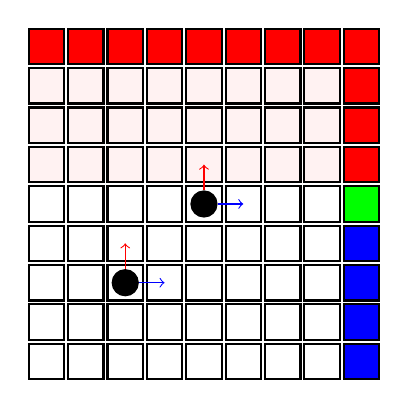
\begin{tikzpicture}
    [%%%%%%%%%%%%%%%%%%%%%%%%%%%%%%
        box/.style={rectangle,draw=black,thick,inner sep=0pt,minimum size=0.45cm},
    ]%%%%%%%%%%%%%%%%%%%%%%%%%%%%%%

\foreach \x in {0,0.5, ..., 4}{
    \foreach \y in {0,0.5, ..., 4}
        \node[box] at (\x,\y){};
}

\foreach \x in {0,0.5, ..., 4}{
        \node[box, fill=red] at (\x,4){};
}

\foreach \y in {2.5,3, ..., 4}{
    \node[box, fill=red] at (4,\y){};
}

\foreach \y in {0,0.5, ..., 1.5}{
    \node[box, fill=blue] at (4,\y){};
} 

\node[box, fill=green] at (4,2){};


\foreach \x in {0,0.5, ..., 3.5}{
    \foreach \y in {2.5,3, ..., 3.5}
        \node[box, fill=red!5] at (\x,\y){};
}
  \node[box] (robot1) at (2,2){};
   \node[box] (robot2) at (1,1){};

  \node[draw, circle, fill=black] (robot11) at (robot1.center) {};
    \node[draw, circle, fill=black] (robot21) at (robot2.center) {};
\draw[->, red] (robot11) -- (2, 2.5);
\draw[->, blue] (robot11) -- (2.5, 2);

\draw[->, red] (robot21) -- (1, 1.5);
\draw[->, blue] (robot21) -- (1.5, 1);
\end{tikzpicture}
\caption{Map of pair-wise synchronizing robots}
\label{fig:map-robots}
\end{figure}
%
Moreover, robot $i$ must synchronize with either robot $i-1$ or $i+1$ (modulo the number of robots) in order to move and both must move with the same direction. Clearly, this would require to create controllers to allow robots to follow that specification. The state of each robot can be modeled by two integers denoting the current position of the robot. We also assume the grid has mines (i.e., bad states) at the top row and the top half most left of the map (i.e., red places in Figure~\ref{fig:map-robots}). 
%
Bottom half most left places are considered safe. Also, we assume that the green location has an exit, which allows the robot to safely exit the map.   

We have modeled robots and their pair-wise synchronization using BIP by allowing them to move to any border locations. Then, we define bad states (i.e., red location) and the goal is to generate a policy that allows robots not go to a bad state. Notice that RE-BIP cannot be used to avoid states as if a robot enters a location on the top half of the map, then 1-step recovery would try all the possible next actions and then fail. For instance, the robot (black circle) on the top has two choices, either moves right or up. The two choices lead the robot to go to a correct state. However, if the robot would take the move up action, it will enter a region where 1-step recovery will fail. 
%
We have tested \rerl using value iteration and deep value iteration by varying the size of the map and the number of robots. Tables~\ref{tab:robots-2},~\ref{tab:robots-4}, \ref{tab:robots-8} depict (1) the success rate when using deep value iteration, value iteration and standard implementation, (2) the time needed to converge in case of deep value iteration, and (3) the number of iterations needed to converge in case of finite value iteration. We ran each configuration $10000$ times to compute the success rate. 
We notice that the value iteration provides a success rate of $100\%$, however, it fails when the size of the system increases. As for the deep value iteration, the system is learning to avoid bad states or states that could lead to bad states and it achieves a high success rate. For instance, if we take a map with $29\times29$ grid size and $8$ robots (i.e., $841^8$ possible states), the standard implementation has $15.1\%$ success rate whereas when using deep value iteration we reach $95.6\%$ success rate. As the state space in this example has a well-defined structure, we only needed $10$ hidden neuron units to train our network by using  deep value iteration algorithm. For this, we notice the efficiency of the compile time, e.g., only $3.6$ seconds are needed to train a system consisting of  $841^8$ states and to reach a $95.6\%$ success rate. 

\begin{table}[t]
\centering
\caption{Evaluation of two robots with different grid sizes.}
{\small
\begin{tabular}{|C{2cm}||C{1.25cm}|C{1.35cm}||C{1.25cm}|C{1.5cm}|C{1.5cm}|}
\hline
\multirow{2}{*}{\textbf{Grid}} & \multicolumn{2}{c||}{\textbf{Infinite}} & \multicolumn{2}{c|}{\textbf{Finite}} & \textbf{Standard}  \\  \cline{2-6}
\textbf{Size} & Succ. \%		& Conv. (s)		&Succ. \% &   Conv. (it.) &    Succ. \%      \\ \hline\hline
\cellcolor{black!10}$5$ & 96.8 & 0.85 &  100 & 7 & 61.7\\ \hline
\cellcolor{black!10}$9$ &	98.6 & 0.98 &	100 & 9& 63.3\\ \hline
\cellcolor{black!10}$13$ &  98.5 & 1.09 &100 & 26& 61.6 \\ \hline
\cellcolor{black!10}$17$ &  99.4 & 1.13 &100 & 34& 58.4\\ \hline
\cellcolor{black!10}$21$ &  99.3 & 1.29 &100 & 42& 63.2\\ \hline
\cellcolor{black!10}$25$ &  99.9 & 1.4 &100 & 50& 59.2\\ \hline
\cellcolor{black!10}$29$  & 99.6 & 1.5 &100 & 58&  61.8\\ \hline
\end{tabular}
}
\label{tab:robots-2}
\end{table}


\begin{table}[t]
\centering
\caption{Evaluation of four robots with different grid sizes.}
{\small
\begin{tabular}{|C{2cm}||C{1.25cm}|C{1.35cm}||C{1.25cm}|C{1.5cm}|C{1.5cm}|}
\hline
\multirow{2}{*}{\textbf{Grid}} & \multicolumn{2}{c||}{\textbf{Infinite}} & \multicolumn{2}{c|}{\textbf{Finite}} & \textbf{Standard}  \\  \cline{2-6}
\textbf{Size} & Succ. \%		& Conv. (s)		&Succ. \% &   Conv. (it.) &    Succ. \%      \\ \hline\hline
\cellcolor{black!10}$5$ & 95.5 & 0.9 &  100 & 7 & 30.5\\ \hline
\cellcolor{black!10}$9$ &	93.9 & 1.08 &	NA & NA& 30.7\\ \hline
\cellcolor{black!10}$13$ &  94.7 & 1.23 &NA & NA& 30.6 \\ \hline
\cellcolor{black!10}$17$ &  97.8 & 1.52 &NA & NA& 28.6\\ \hline
\cellcolor{black!10}$21$ &  97.9 & 1.82 &NA & NA& 29.8\\ \hline
\cellcolor{black!10}$25$ &  98.1 & 2.2 &NA & NA& 30.1\\ \hline
\cellcolor{black!10}$29$  & 97.8 & 2.5 &NA & NA&  30.1\\ \hline
\end{tabular}
}
\label{tab:robots-4}
\end{table}

\begin{table}[t]
\centering
\caption{Evaluation of eight robots with different grid sizes.}
{\small
\begin{tabular}{|C{2cm}||C{1.25cm}|C{1.35cm}||C{1.25cm}|C{1.5cm}|C{1.5cm}|}
\hline
\multirow{2}{*}{\textbf{Grid}} & \multicolumn{2}{c||}{\textbf{Infinite}} & \multicolumn{2}{c|}{\textbf{Finite}} & \textbf{Standard}  \\  \cline{2-6}
\textbf{Size} & Succ. \%		& Conv. (s)		&Succ. \% &   Conv. (it.) &    Succ. \%      \\ \hline\hline
\cellcolor{black!10}$5$ & 92.9 & 1.1 &  NA & NA & 12.2\\ \hline
\cellcolor{black!10}$9$ &	93.9 & 1.5 &	NA & NA& 13.8\\ \hline
\cellcolor{black!10}$13$ &  97.4 & 1.6 &NA & NA& 15.1 \\ \hline
\cellcolor{black!10}$17$ &  95.3 & 2.2 &NA & NA& 13.8\\ \hline
\cellcolor{black!10}$21$ &  94.9 & 3.0 &NA & NA& 17.1\\ \hline
\cellcolor{black!10}$25$ &  94.8 & 3.3 &NA & NA& 14.2\\ \hline
\cellcolor{black!10}$29$  & 95.6 & 3.6 &NA & NA&  15.1\\ \hline
\end{tabular}
}
\label{tab:robots-8}
\end{table}

